\section{Experimental Design}
\label{sec:design}
\label{sec:experiments}

The immutable C1.2 matrix crosses task counts $\{12,18\}$, four synthetic stress levels, and held-out seeds $\{101,211,307,401\}$ for 32 instances. Development seeds 11 and 23 are excluded. Each instance uses 24 correlated scenarios, three regions, three-task workflow clusters, service target .70, chance tolerance .20, review capacity, and a four-task retained core. QAOA depths $p=1,2$ are frozen; $p=1$ receives a $13\times11=143$-point grid and $p=2$ receives 30 seeded random trials, so depth comparisons are descriptive rather than an equal-optimizer-budget ablation.

Uniform and $p=2$ retained-core probabilities each receive 128 draws. Prespecified outcomes include strict-core availability, classical gain and ambiguity, optimum mass, first-hit draw (miss coded 129), near-optimal coverage, gate status, composite feasibility, and disallowed-mode violations. Percentile 95\% bootstrap intervals resample paired instances 10,000 times. Sampling probability, best-of-budget assignment, practical runtime, application outcomes, and welfare remain distinct estimands.

\paragraph{Resource account and reproducibility boundary.}
Matched draws answer a narrow sampling question: given two retained-state distributions and 128 samples from each, how often is an optimum observed? They do not match the work required to construct the retained core, enumerate strict states, optimize QAOA parameters, simulate a statevector, communicate with hardware, verify candidates, or recover from failure. The $p=1$ grid and $p=2$ random search are also unequal optimization budgets. We therefore report sampling probability separately from best-of-budget assignment quality and exclude runtime, energy, and cost conclusions. The frozen configuration and null-inclusive development history implement a reproducibility discipline in which negative stages are evidence rather than discarded tuning attempts~\citep{pineau2021reproducibility}. Reproduction here means executing the same code and data under documented conditions; it is not an independent replication on new instances or another implementation.

The development sequence is preserved rather than rewritten as a success-only narrative. C1.0 left too little useful headroom after strong classical search. C1.1 showed probability concentration without jointly establishing strict feasibility and classical ambiguity. C1.2 froze feasibility, headroom/ambiguity, matched retained-state comparison, selective gating, a quantum-independent classical verification boundary, and fallback before the held-out run. \Cref{fig:evolution} shows why each control is necessary; only C1.2 carries headline numbers.

\begin{figure*}[t]
\centering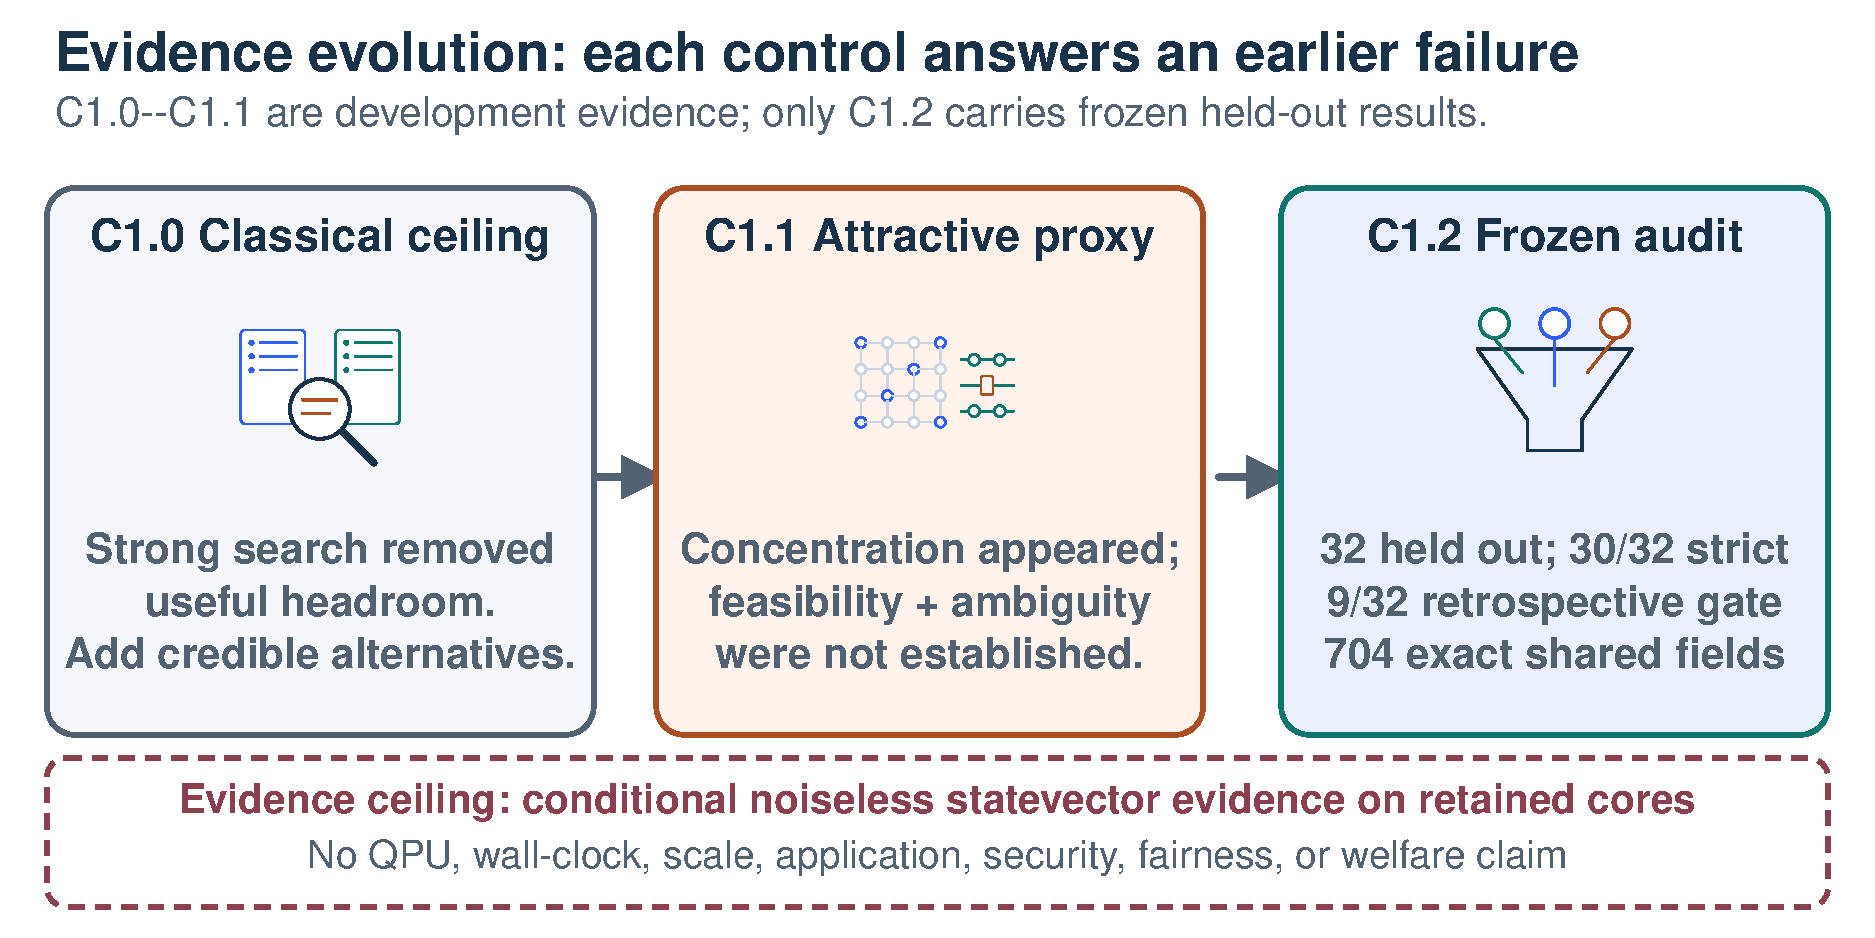
\includegraphics[width=\textwidth]{figs/fig3_evidence_evolution.pdf}
\caption{\textbf{Evidence evolution as a control argument.} C1.0 shows why credible classical alternatives are necessary; C1.1 shows why concentration alone is insufficient; C1.2 freezes strict feasibility, ambiguity/headroom, matched draws, a recorded gate, shared verification, and fallback. Only the immutable C1.2 held-out evaluation supplies headline numbers.}\label{fig:evolution}
\end{figure*}


A fresh runner produced 32 rows. Across the 22 shared fields and 32 records, all 704 comparisons match the archived table exactly (maximum absolute error 0). Eight archived diagnostics are no longer emitted, so the claim is exact \emph{shared-field} reproduction, not byte-identical CSV reproduction. New router baselines, gate ablations, risk--coverage curves, QPU runs, and stronger full-problem solvers were not reproducible from the frozen protocol without changing the study; they are therefore preregistered evaluation priorities rather than fabricated results. The configuration digest and full environment record appear in Appendix~\ref{app:protocol}.
